
%%%%%%%%%%%%%%%%%%%%%%% file typeinst.tex %%%%%%%%%%%%%%%%%%%%%%%%%
%
% This is the LaTeX source for the instructions to authors using
% the LaTeX document class 'llncs.cls' for contributions to
% the Lecture Notes in Computer Sciences series.
% http://www.springer.com/lncs       Springer Heidelberg 2006/05/04
%
% It may be used as a template for your own input - copy it
% to a new file with a new name and use it as the basis
% for your article.
%
% NB: the document class 'llncs' has its own and detailed documentation, see
% ftp://ftp.springer.de/data/pubftp/pub/tex/latex/llncs/latex2e/llncsdoc.pdf
%
%%%%%%%%%%%%%%%%%%%%%%%%%%%%%%%%%%%%%%%%%%%%%%%%%%%%%%%%%%%%%%%%%%%


\documentclass[runningheads,a4paper]{llncs}

\usepackage{amssymb}
\setcounter{tocdepth}{3}
\usepackage{graphicx}
\usepackage{float}
\usepackage[full]{complexity}
\usepackage{amsmath}
%\usepackage{amsfonts}
%\usepackage{amsthm}
\usepackage{subfigure}
%\usepackage{caption}
%\usepackage{subcaption}
%\usepackage{cite}
\usepackage{hyperref}
\usepackage{url}
\usepackage{clrscode4e}
\usepackage{verbatim}
\urlstyle{same}
\newcommand{\keywords}[1]{\par\addvspace\baselineskip
\noindent\keywordname\enspace\ignorespaces#1}

% Uniform numbering for previously defined theorem environments (e.g., LNCS).
\makeatletter
\let\c@lemma=\c@theorem
\let\c@corollary=\c@theorem
\let\c@fact=\c@theorem
\makeatother

% Redefinition of LNCS or SODA or Springer proof environment to put a \Box at
% the end of every proof.
\let\realendproof=\endproof
\def\endproof{\hspace*{\fill}$\Box$\realendproof}

\begin{document}

\mainmatter  % start of an individual contribution

% first the title is needed
\title{The Complexity of Determining Critical Sets}

% a short form should be given in case it is too long for the running head
\titlerunning{The Complexity of Determining Critical Sets}

% the name(s) of the author(s) follow(s) next
%
% NB: Chinese authors should write their first names(s) in front of
% their surnames. This ensures that the names appear correctly in
% the running heads and the author index.
%
\author{Fermi Ma \and Ariel Schvartzman \and Erik Waingarten}
%
\authorrunning{Fermi Ma \and Ariel Schvartzman \and Erik Waingarten}
% (feature abused for this document to repeat the title also on left hand pages)

% the affiliations are given next; don't give your e-mail address
% unless you accept that it will be published
\institute{MIT,\\
77 Mass Ave., Cambridge, MA 02139, USA, \\
\protect\url{{fermima,arielsc,eaw}@mit.edu}}

%
% NB: a more complex sample for affiliations and the mapping to the
% corresponding authors can be found in the file "llncs.dem"
% (search for the string "\mainmatter" where a contribution starts).
% "llncs.dem" accompanies the document class "llncs.cls".
%

\maketitle

\section{SAT}
\begin{itemize}
\item $f$ is the Cook-Levin construction, and add variables $a_{l, q, i, j, k}$ to indicate whether took left branch at time $k$ from state $q$ and wrote at $i$ character $j$. 
\item $C_B'$ is the set of clues involving only true values of $a_{l,q,i,j,k}$ and full solutions.
\item $M$ takes variables which are false and finds the ones that are true. This is done in polytime since a variable being true, implies one being false. We know that one must be true, so we can look for it. $M$ sets $a_{l,q,i,j,k}$ while removing other variables.
\item $g$ sends $a_{l,q,i,j,k}$ which is true into took $l$ branch at time $k$.
\end{itemize}

Note that algorithm $M$ takes minimal to minimal since any false variable can be replaced, and any non-$a$ variable can be replaced with an $a$ variable which implies it. 

$g$is surjective, since for each right-branch, left-branch, there exists a set of $a$'s set to True. $g$ is bijective on the solutions since Cook-Levin is parsimonious. If $c_1 \subset c_2$, then $g(c_1) \subset g(c_2)$ since $g$ maps each element for $c$.

\section{3SAT}

\begin{itemize}
\item $f$ takes all clauses like this: if below $4$ variables, then the obvious. If clause $C$ has $n$ variables, $x_1, ..., x_n$, then map to
\[ (x_1 \vee x_2 \vee z_2) \wedge (\overline{z_2} \vee \overline{x_2}) \wedge (z_2 \vee x_2) \wedge f(\overline{z_2}, x_3, ..., x_n) \]
\item $C_B'$ is the set of clues involving $x_i$ and full solutions.
\item $M$: switch $z_i$ to $x_i$.
\item $g$ projects
\end{itemize}

Note that $f$ works, and its parsimonious. $M$ takes a minimal to a minimal since we add an element and remove an element. 

$g$ is actually bijective, since $x_i \leftrightarrow z_i$. Subsets hold since $g$ maps individual elements.

\subsection{NAE-3SAT}

Note that the same reduction holds, since the instance created will never have all the elements in a clause set to true. 

\subsection{1-in-3 SAT}

Also, we if we add the modification to the above reduction where instead of $(x_1 \vee x_2 \vee z_2)$, we write $(x_1 \vee z_1) \wedge (\overline{z_1} \vee \overline{x_1}) \wedge (\overline{z_1} \vee x_2 \vee z_2)$, then we never have more than one thing set to true in each clause. 

Therefore, this reduction would show that $\mathsf{FCP}$ 1-in-3SAT is $\mathsf{FCP}$-hard. 

\section{Triangle Partition}

\begin{itemize}
\item $f$ is Holyer construction.
\item $C_B$ is the clues with at most one particular triangle per $H_{3,p}$ graph, not in unions, the first true literal of each clause is set to $F$-partition. 
\item $M$ translates the triangles to particular triangle. It also moves the triangles in the clauses so that the first true literal is set $F$-partition.
\item $g$ projects variables. 
\end{itemize}

Note that $M$ is fine becuase if a clause is set to $T$ partition, it doesn't add information, so we put whichever literal to $F$ partition that we need. 

$g$ is a surjection since it projects. $g$ is also a bijection on solutions since we defined designated how $C_B'$ will assign clauses in light of ambiguity. $g$ preserves subsets since each element maps to another element. 

\section{Latin Squares}

\begin{itemize}
\item $f$ is the reduction which maps to the defect graph.
\item sets of triangles correspond to numbers, so $C_B'$ is the same. 
\end{itemize}

\section{Sudoku}

\begin{itemize}
\item $f$ blows up the size of the Latin Squares problem as in this figure:  
\begin{figure}[H]
\label{fig:partialLS}
\centering
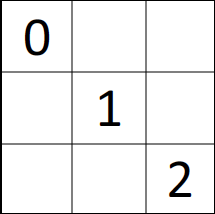
\includegraphics[scale=0.25]{sudoku-3.png}
\end{figure}

\begin{figure}[H]
\label{fig:partialNP}
\centering
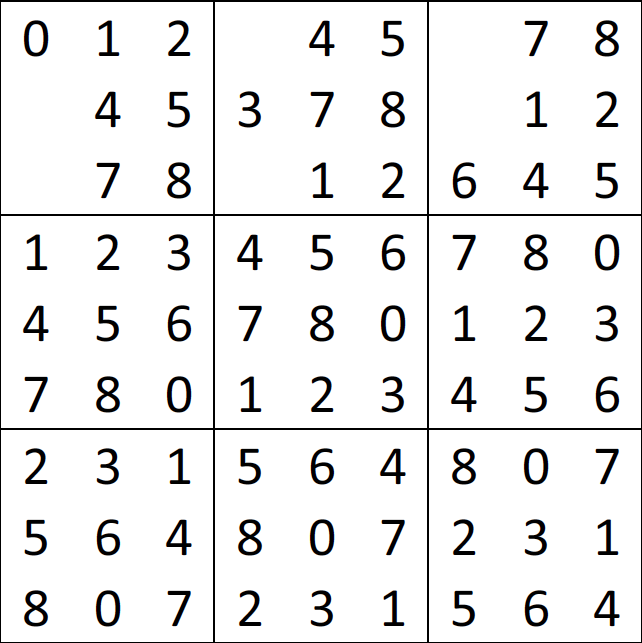
\includegraphics[scale=0.25]{sudoku-1.png}
\end{figure}
\item $C_B$ is the total set of clues.
\item $M$ does nothing.
\item $g$ projects the clues in the only way.
\end{itemize}

Note that $g$ is surjective, since the reduction gives us a Sudoku. $g$ is bijective on everything and since it maps elements, it preserves subsets. 

\section{3-colorability}

We have a reduction from 3SAT. 
\begin{figure}
\centering
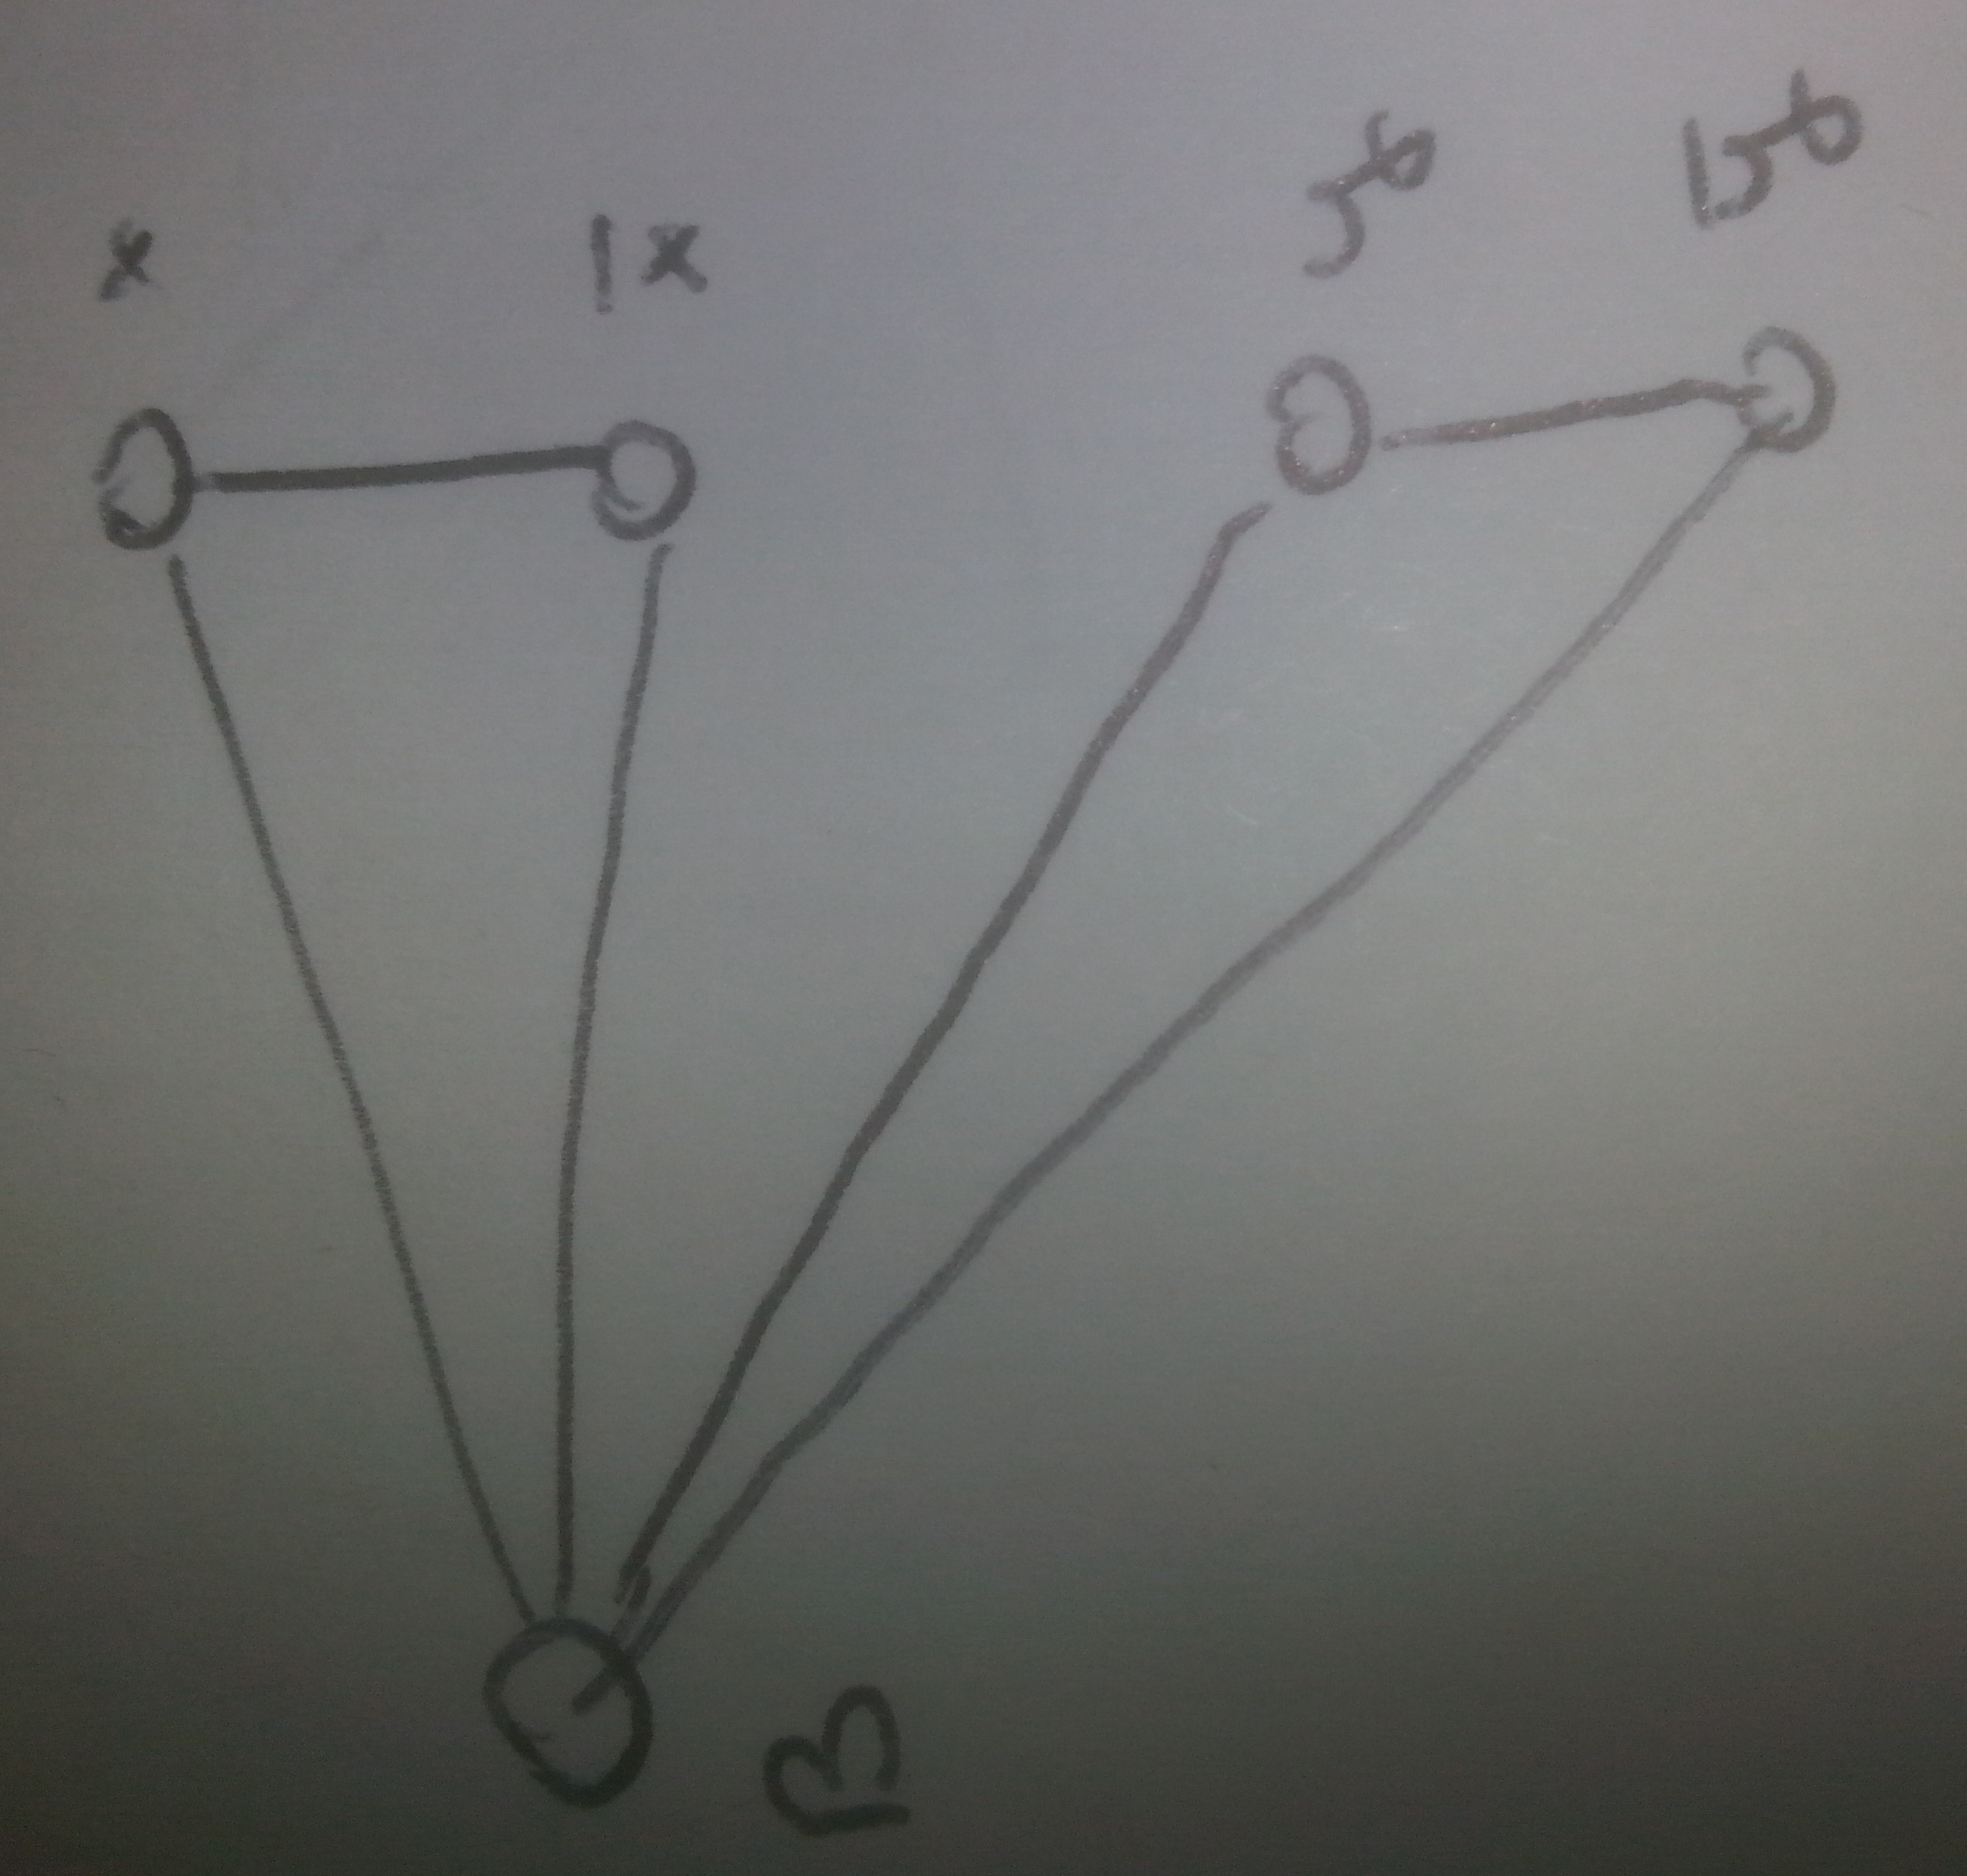
\includegraphics[width=0.3\linewidth, angle=-90]{3colorable-var.jpg}
\caption{variable gadget}
\end{figure}

\begin{figure}
\centering
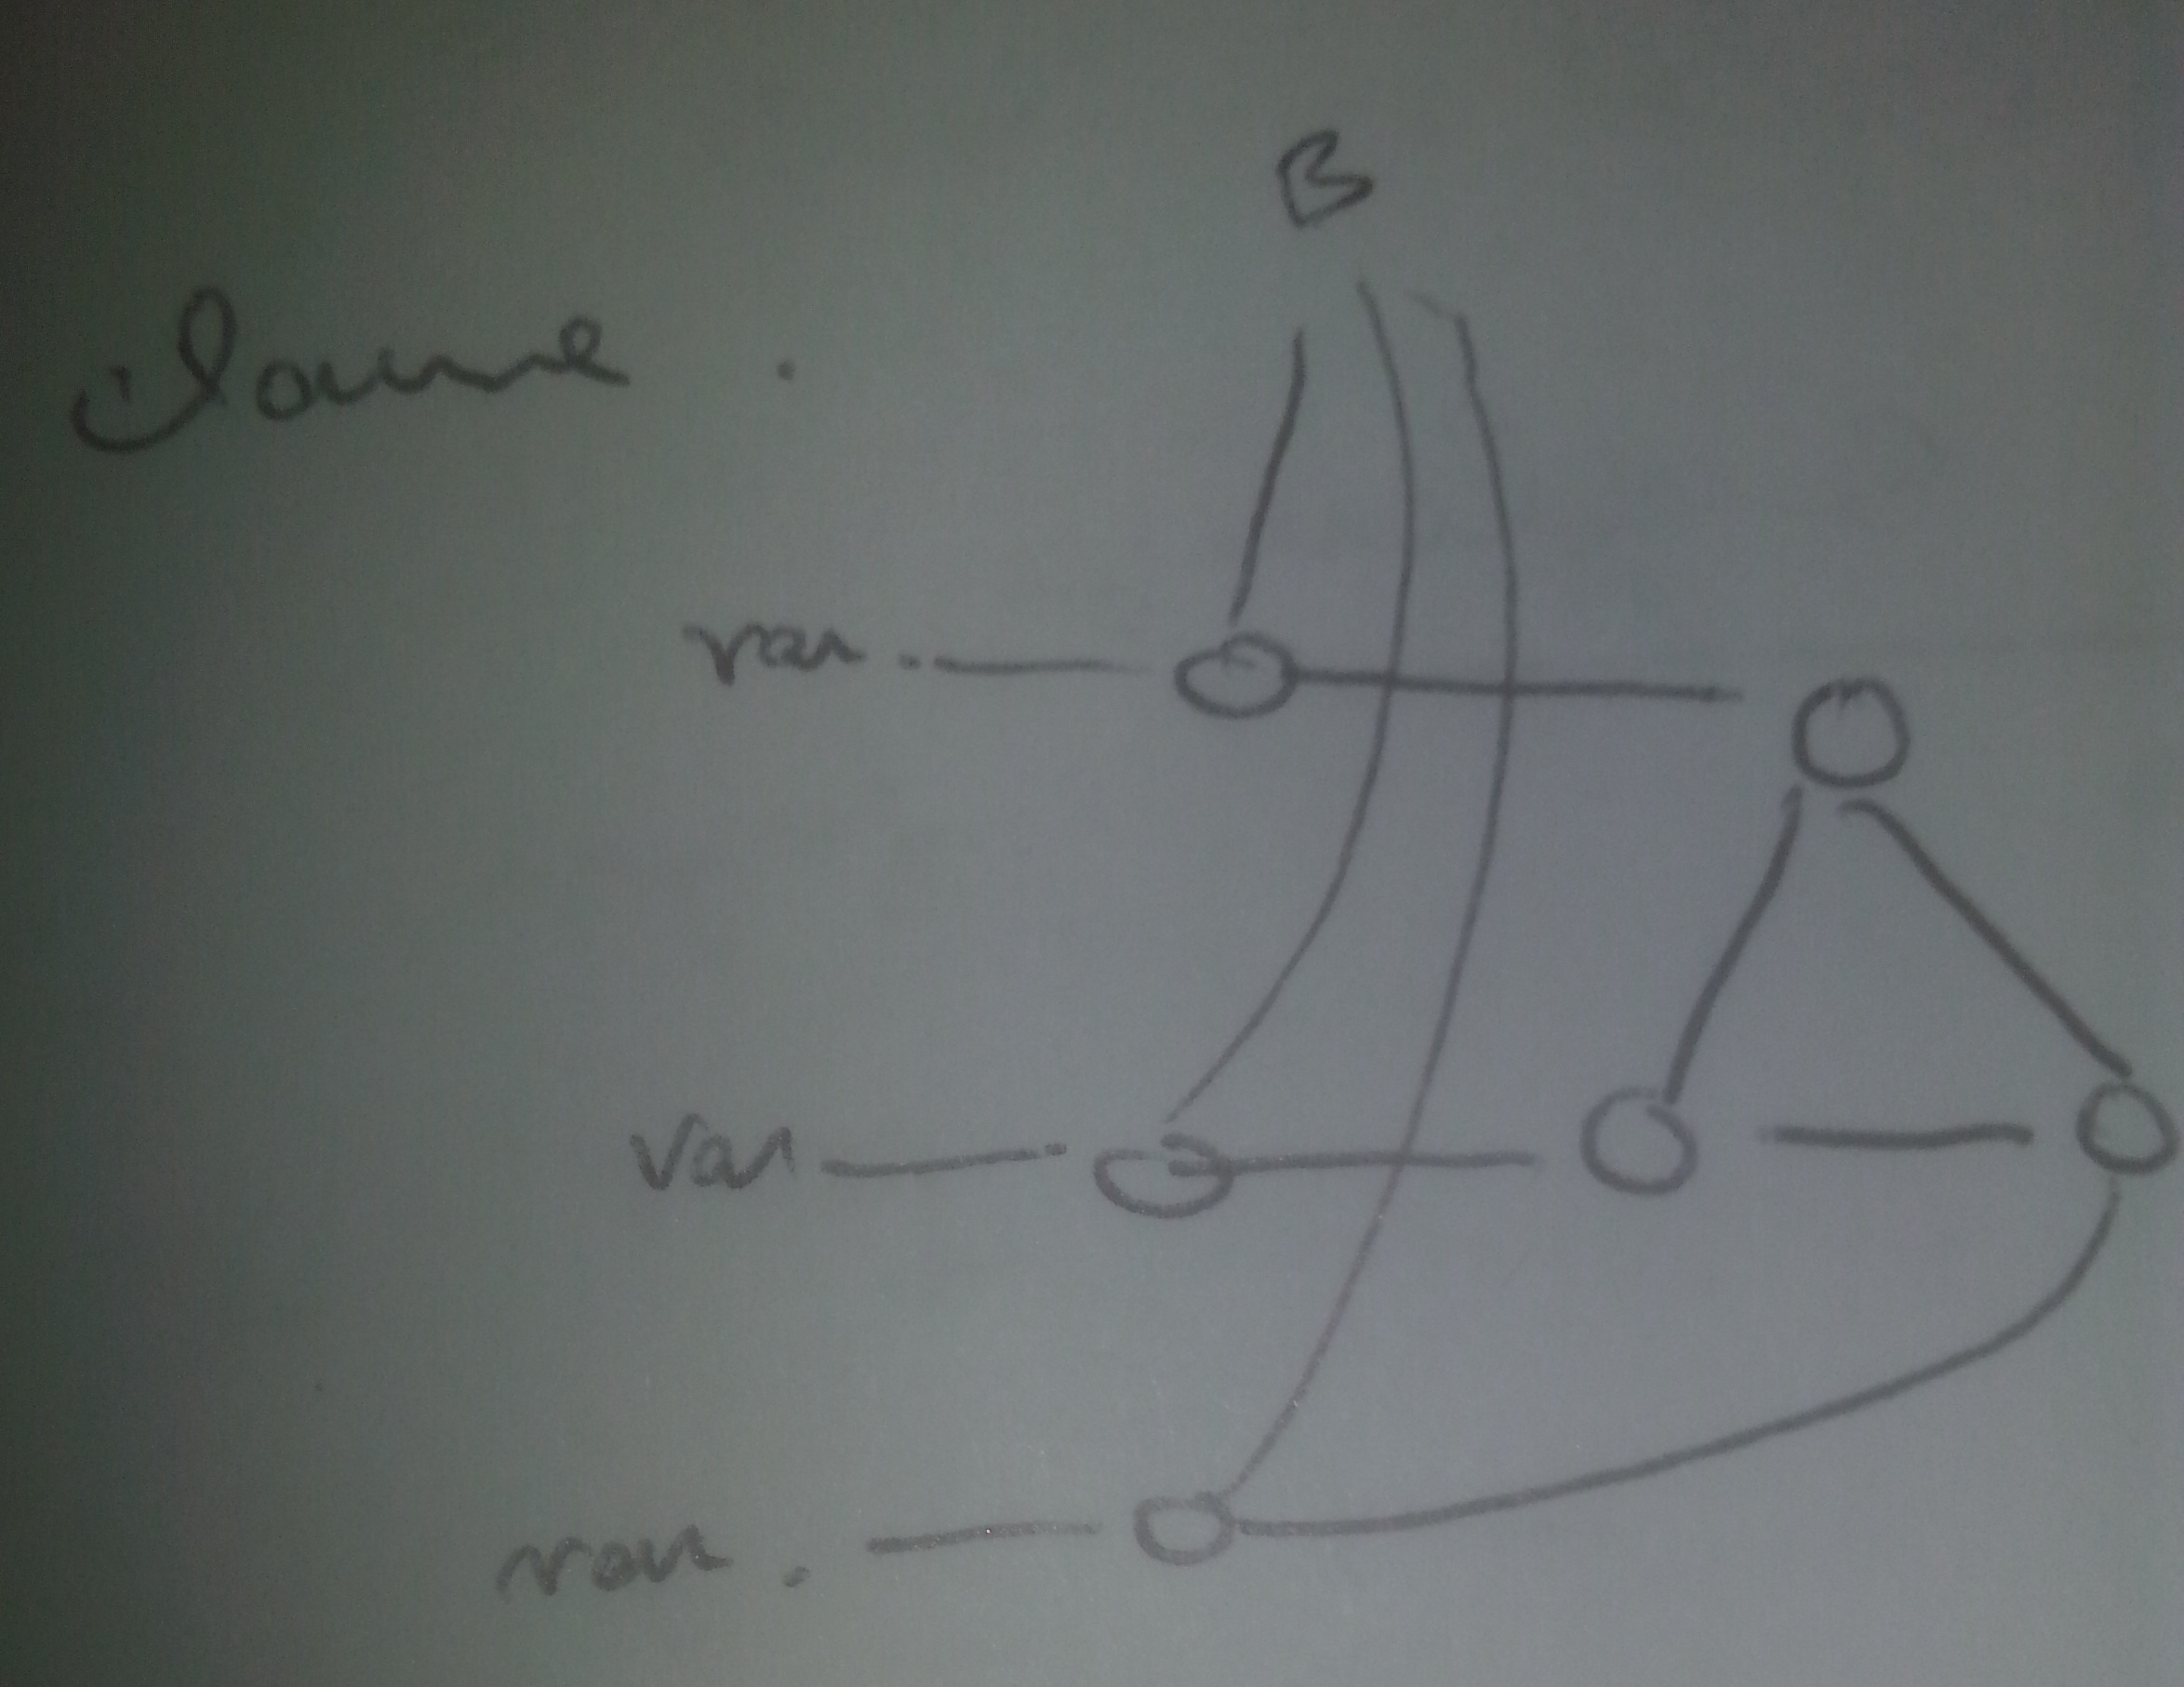
\includegraphics[width=0.3\linewidth]{3colorable-clause.jpg}
\caption{clause gadget}
\end{figure}

Now we can do a similar thing as in triangle partition and make the F colors in the clause be the first ones written out. We also note that this throws away information, so it makes sense that it is still $\mathsf{FCP}$-hard. Furthermore, if the formula is planar, then the graph can be turned planar, with the following transformation, where also we keep alternating up between $x, \overline{x}, x, \overline{x}, ... $ so that each appearence connects to one, and since these are connected in a path (also all to $B$), they will have the same color.

\begin{figure}
\centering
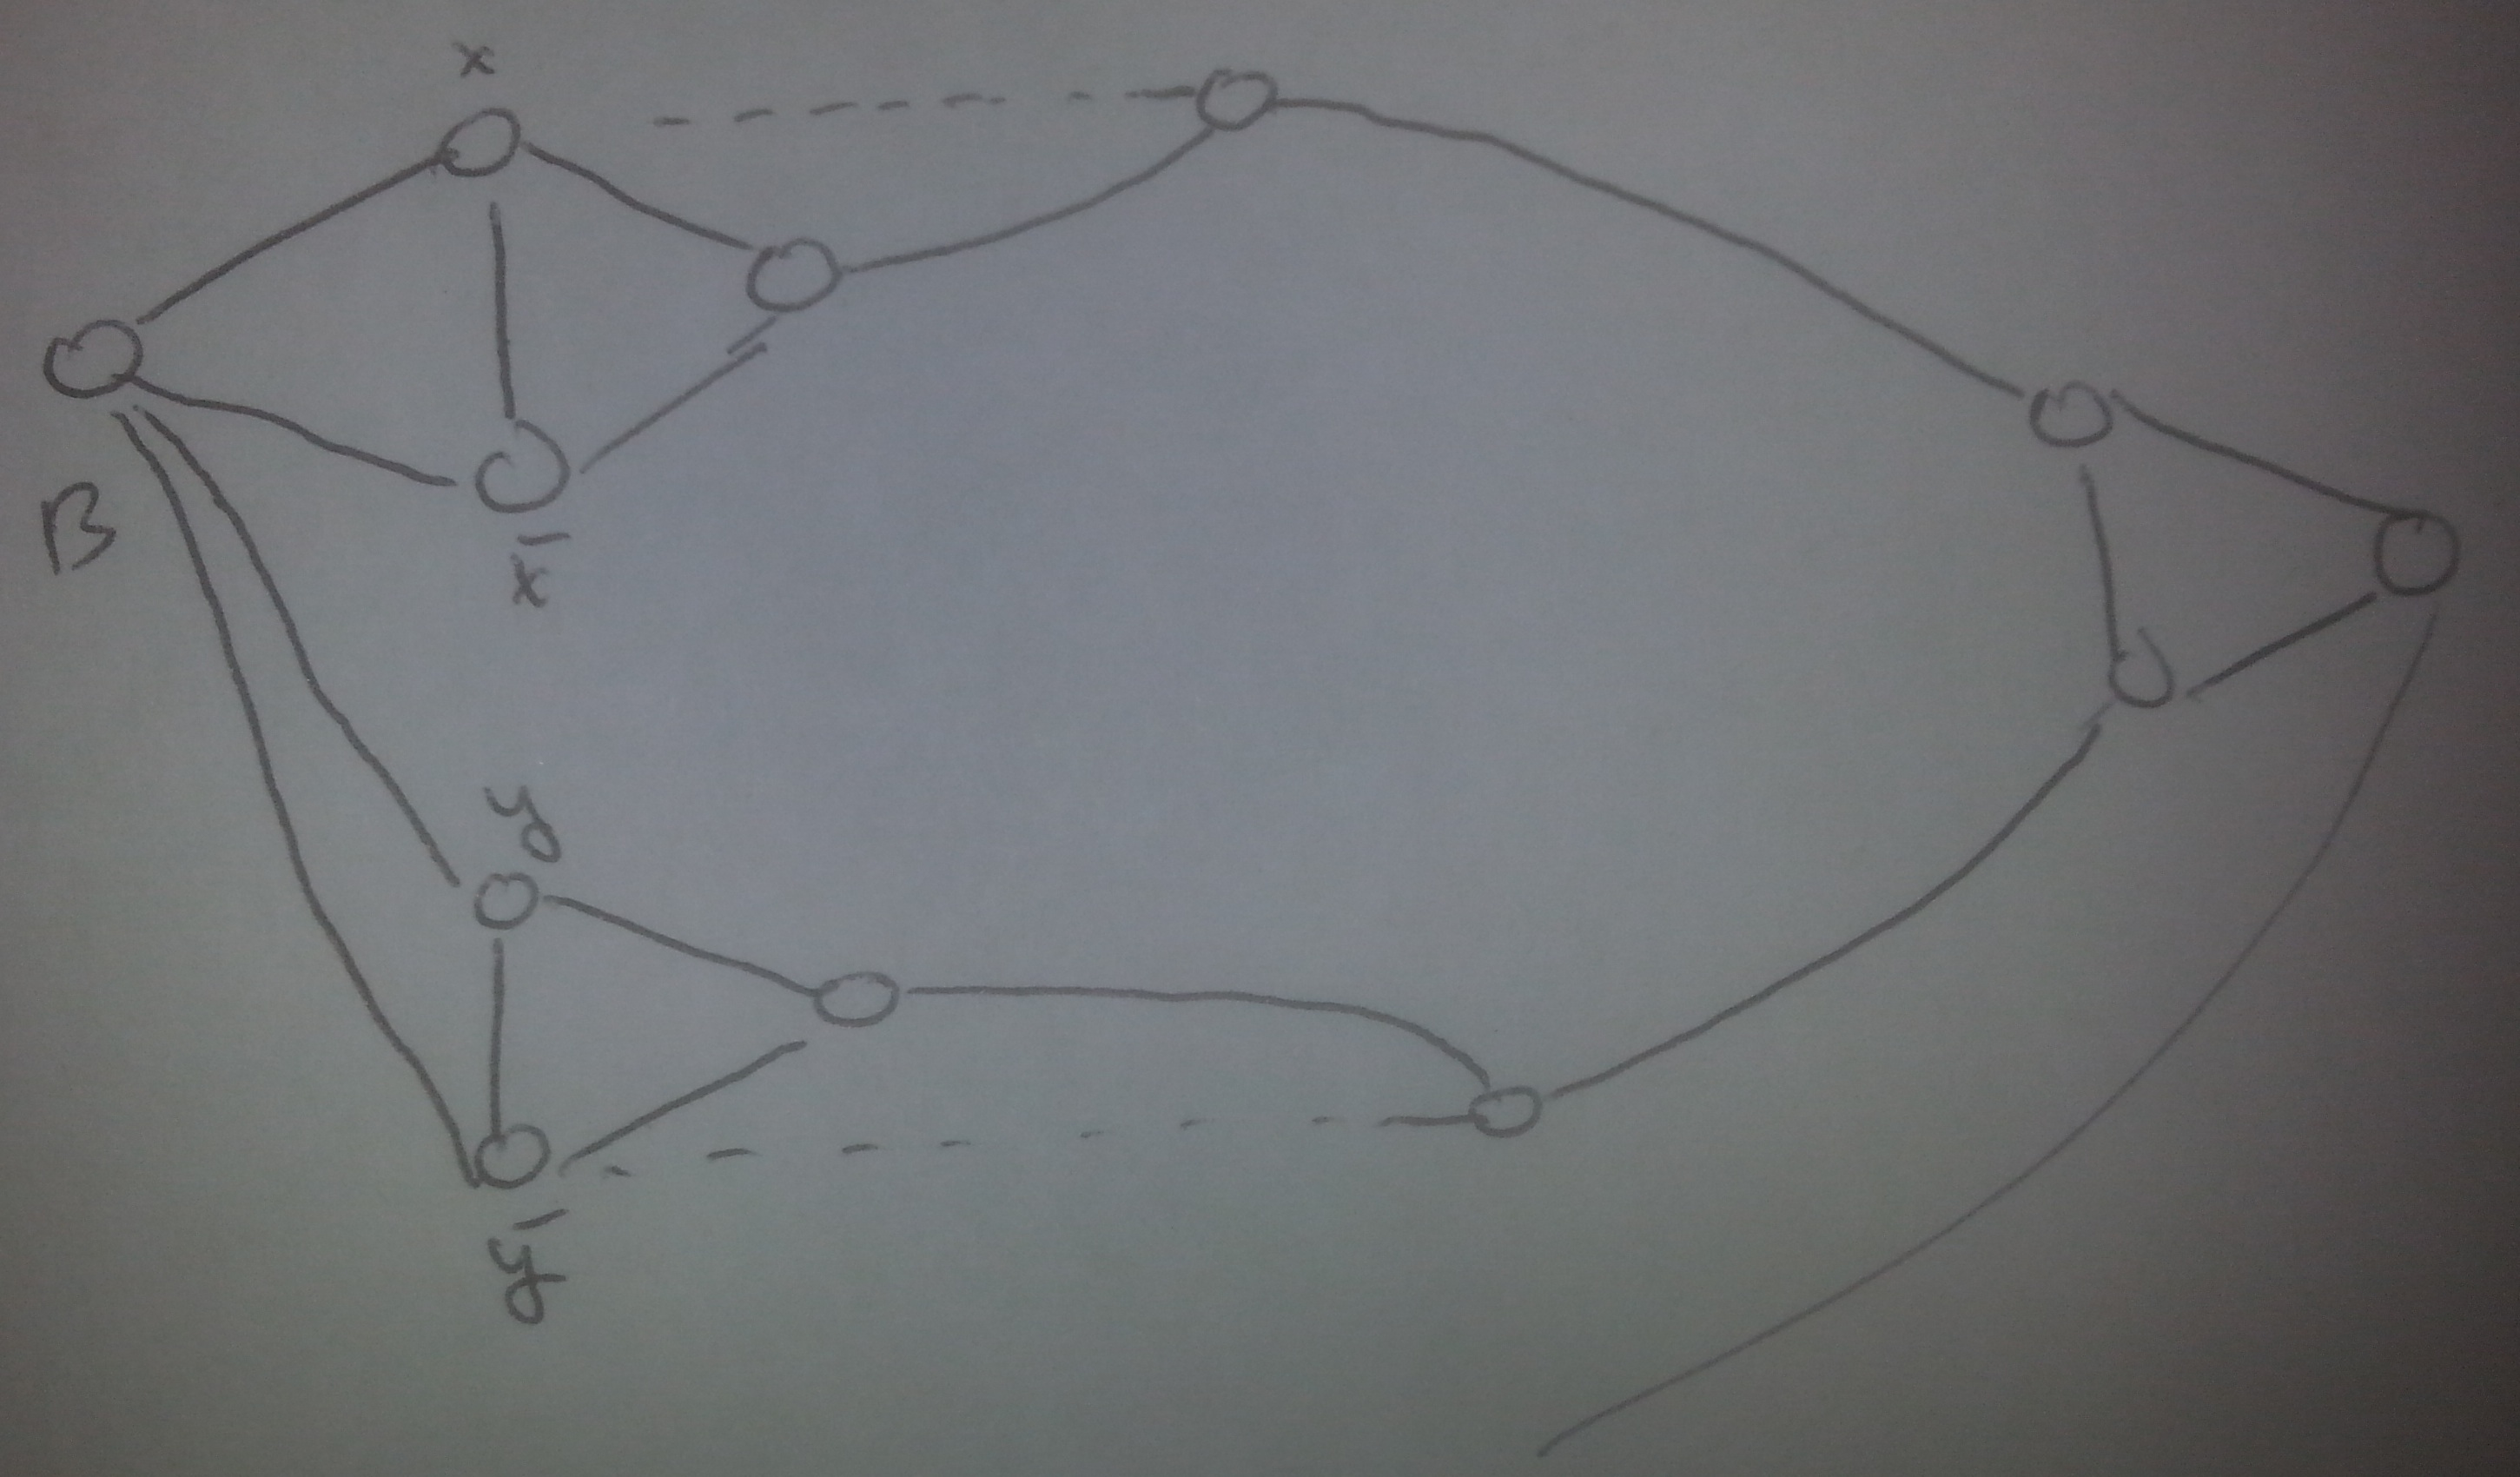
\includegraphics[width=0.4\linewidth]{3colorable-planar.jpg}
\caption{making the reduction planar}
\end{figure}

\section{Bag - Corral}

If we assume that planar 3-coloring is $\mathsf{FCP}$-hard, then Corral is $\mathsf{FCP}$-hard. The clues here are lists of edges that are included in the graph. We can use the reduction from \url{http://www2.stetson.edu/~efriedma/papers/corral/corral.html} and note that since for each wire there are three possible fillings, the clues can be moved, and each implies the next, until we get to a turn (in particular, this corresponds to the edges that border the colors, but not true ones. Therefore, we can move the final solution to the values of the vertices. And so we can  three-color the graph, since in a vertex, we know how to color them since we know which edge starts the signal.

\section{Indepedent set}

Trivial. Using reduction from \url{https://www.cs.cmu.edu/~ckingsf/bioinfo-lectures/sat.pdf}

\end{document}
